\documentclass{standalone}
\usepackage{tikz}
\usetikzlibrary{patterns}
\usetikzlibrary{positioning}
\usetikzlibrary{patterns, positioning}
\usetikzlibrary{shapes.misc}
\usepackage[outline]{contour}
\contourlength{1.5pt} 
\usepackage[sfdefault]{ClearSans}

\begin{document}
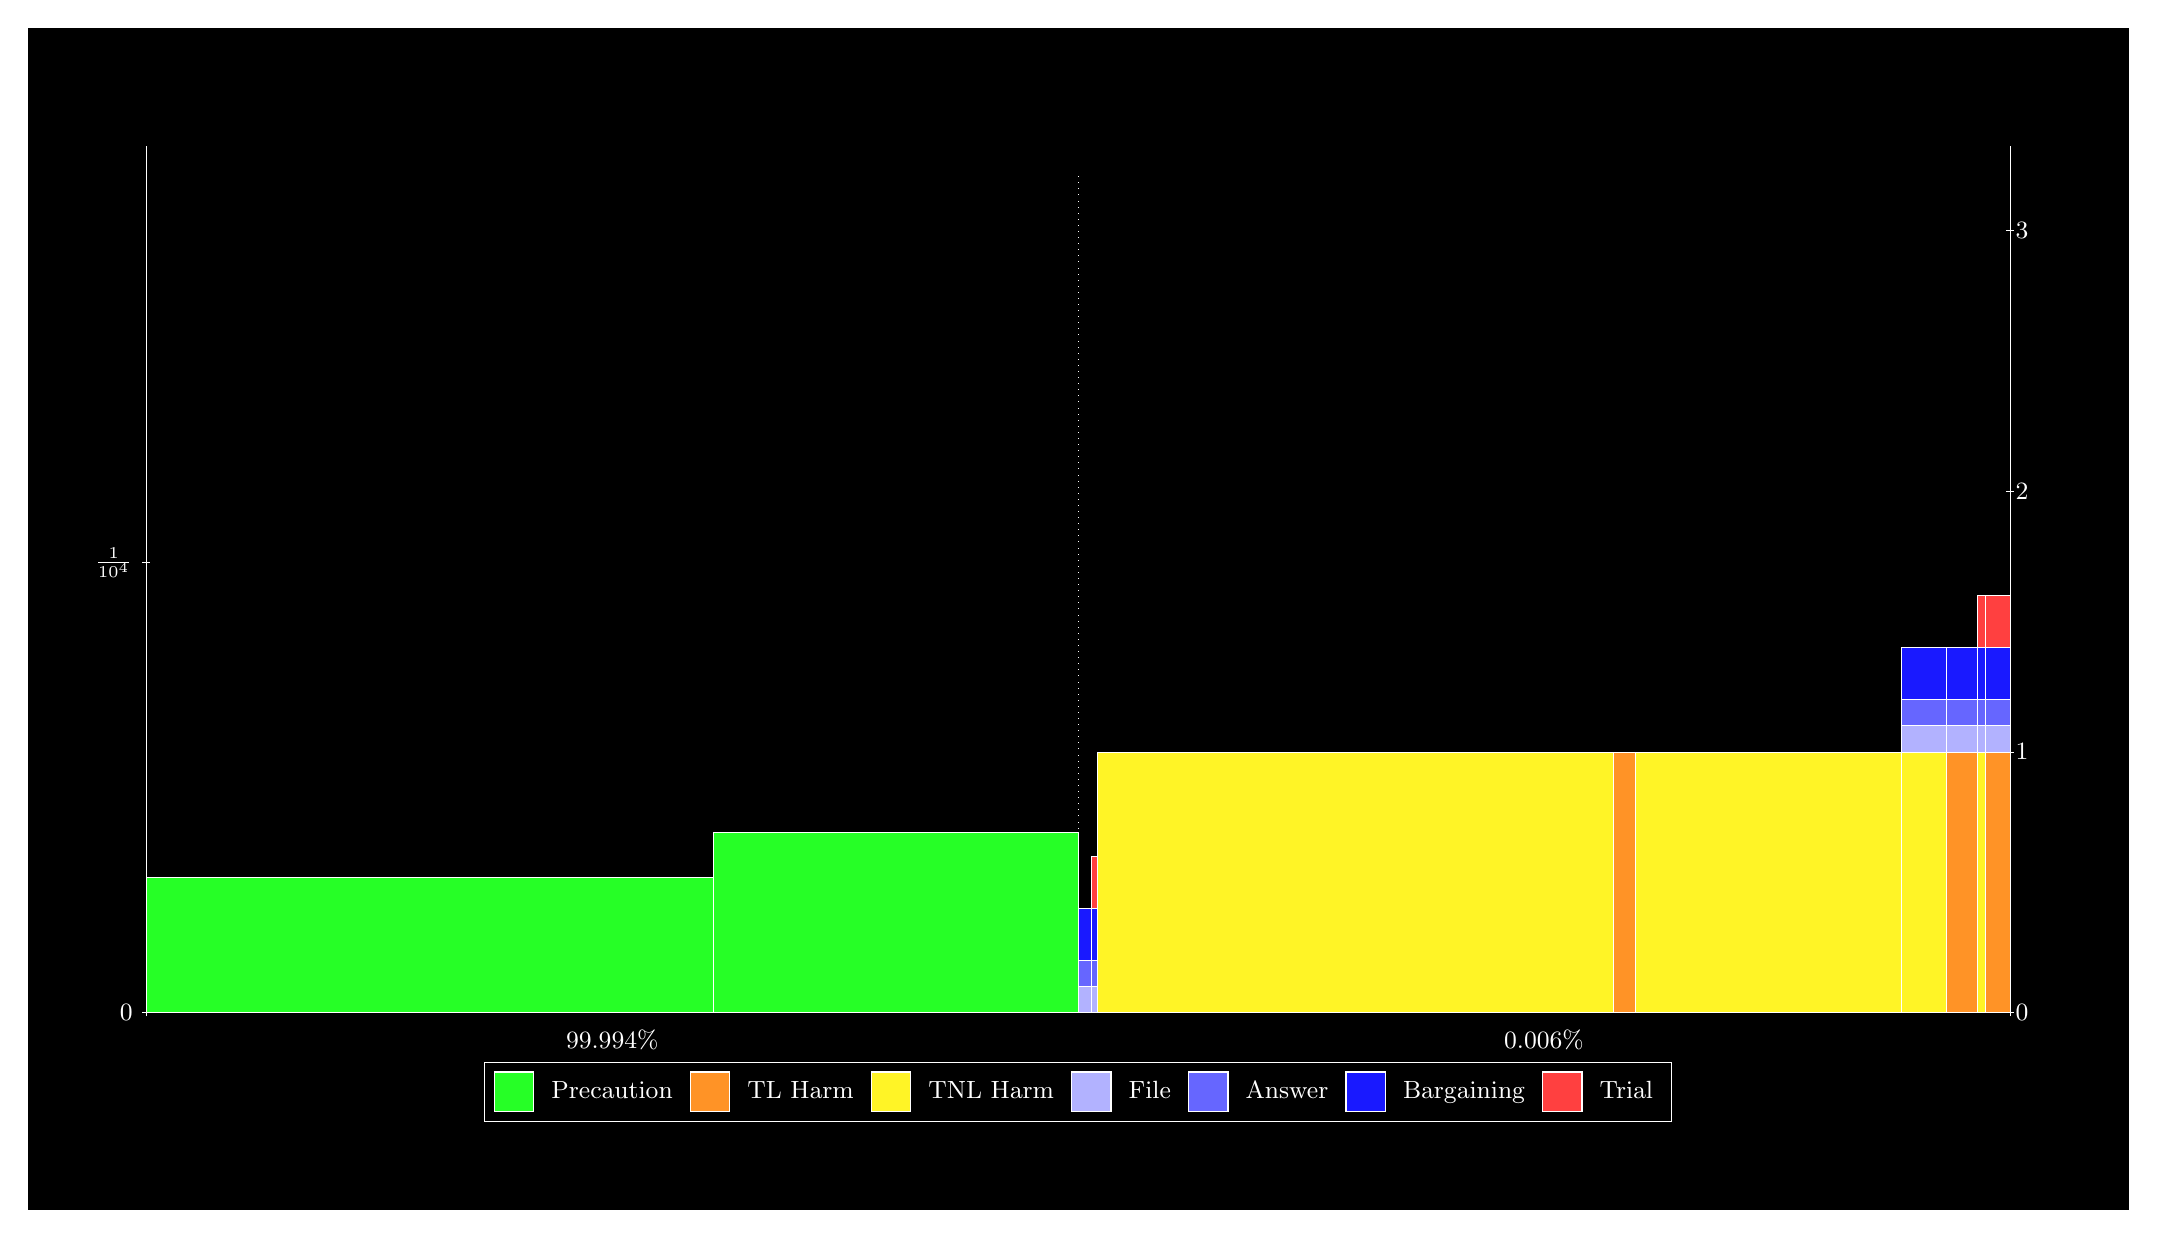
\begin{tikzpicture}
\draw[fill=black] (0,0) rectangle (26.667,15);
\draw[fill=green!85,draw=white,very thin] (1.5,2.5) rectangle (8.696,4.2142);
\draw[fill=green!85,draw=white,very thin] (8.696,2.5) rectangle (13.333,4.7856);
\draw[fill=green!85,draw=white,very thin] (13.333,2.5) rectangle (13.5,2.5001);
\draw[fill=blue!30,draw=white,very thin] (13.333,2.5001) rectangle (13.5,2.8311);
\draw[fill=blue!60,draw=white,very thin] (13.333,2.8311) rectangle (13.5,3.1622);
\draw[fill=blue!90,draw=white,very thin] (13.333,3.1622) rectangle (13.5,3.8242);
\draw[fill=green!85,draw=white,very thin] (13.5,2.5) rectangle (13.577,2.5001);
\draw[fill=blue!30,draw=white,very thin] (13.5,2.5001) rectangle (13.577,2.8311);
\draw[fill=blue!60,draw=white,very thin] (13.5,2.8311) rectangle (13.577,3.1622);
\draw[fill=blue!90,draw=white,very thin] (13.5,3.1622) rectangle (13.577,3.8242);
\draw[fill=red!75,draw=white,very thin] (13.5,3.8242) rectangle (13.577,4.4863);
\draw[fill=green!85,draw=white,very thin] (13.577,2.5) rectangle (20.133,2.5001);
\draw[fill=yellow!85,draw=white,very thin] (13.577,2.5001) rectangle (20.133,5.8105);
\draw[fill=green!85,draw=white,very thin] (20.133,2.5) rectangle (20.405,2.5001);
\draw[fill=orange!85,draw=white,very thin] (20.133,2.5001) rectangle (20.405,5.8105);
\draw[fill=green!85,draw=white,very thin] (20.405,2.5) rectangle (23.791,2.5001);
\draw[fill=yellow!85,draw=white,very thin] (20.405,2.5001) rectangle (23.791,5.8105);
\draw[fill=green!85,draw=white,very thin] (23.791,2.5) rectangle (24.363,2.5001);
\draw[fill=yellow!85,draw=white,very thin] (23.791,2.5001) rectangle (24.363,5.8105);
\draw[fill=blue!30,draw=white,very thin] (23.791,5.8105) rectangle (24.363,6.1415);
\draw[fill=blue!60,draw=white,very thin] (23.791,6.1415) rectangle (24.363,6.4725);
\draw[fill=blue!90,draw=white,very thin] (23.791,6.4725) rectangle (24.363,7.1346);
\draw[fill=green!85,draw=white,very thin] (24.363,2.5) rectangle (24.758,2.5001);
\draw[fill=orange!85,draw=white,very thin] (24.363,2.5001) rectangle (24.758,5.8105);
\draw[fill=blue!30,draw=white,very thin] (24.363,5.8105) rectangle (24.758,6.1415);
\draw[fill=blue!60,draw=white,very thin] (24.363,6.1415) rectangle (24.758,6.4725);
\draw[fill=blue!90,draw=white,very thin] (24.363,6.4725) rectangle (24.758,7.1346);
\draw[fill=green!85,draw=white,very thin] (24.758,2.5) rectangle (24.86,2.5001);
\draw[fill=yellow!85,draw=white,very thin] (24.758,2.5001) rectangle (24.86,5.8105);
\draw[fill=blue!30,draw=white,very thin] (24.758,5.8105) rectangle (24.86,6.1415);
\draw[fill=blue!60,draw=white,very thin] (24.758,6.1415) rectangle (24.86,6.4725);
\draw[fill=blue!90,draw=white,very thin] (24.758,6.4725) rectangle (24.86,7.1346);
\draw[fill=red!75,draw=white,very thin] (24.758,7.1346) rectangle (24.86,7.7967);
\draw[fill=green!85,draw=white,very thin] (24.86,2.5) rectangle (25.167,2.5001);
\draw[fill=orange!85,draw=white,very thin] (24.86,2.5001) rectangle (25.167,5.8105);
\draw[fill=blue!30,draw=white,very thin] (24.86,5.8105) rectangle (25.167,6.1415);
\draw[fill=blue!60,draw=white,very thin] (24.86,6.1415) rectangle (25.167,6.4725);
\draw[fill=blue!90,draw=white,very thin] (24.86,6.4725) rectangle (25.167,7.1346);
\draw[fill=red!75,draw=white,very thin] (24.86,7.1346) rectangle (25.167,7.7967);
\draw[white,very thin] (1.5,2.5) -- (1.5,13.5);
\draw[white,very thin] (1.45,2.5) -- (1.55,2.5);
\node[font=\small,text=white, anchor=east] at (1.45, 2.5) {0};
\draw[white,very thin] (1.45,8.214) -- (1.55,8.214);
\node[font=\small,text=white, anchor=east] at (1.45, 8.214) {$\frac{1}{10^{4}}$};

\draw[white,dotted,very thin] (13.333,2.83) -- (13.333,13.17);
\draw[white,very thin] (25.167,2.5) -- (25.167,13.5);
\draw[white,very thin] (25.117,2.5) -- (25.217,2.5);
\node[font=\small,text=white, anchor=west] at (25.117, 2.5) {0};
\draw[white,very thin] (25.117,5.8104) -- (25.217,5.8104);
\node[font=\small,text=white, anchor=west] at (25.117, 5.8104) {1};
\draw[white,very thin] (25.117,9.1207) -- (25.217,9.1207);
\node[font=\small,text=white, anchor=west] at (25.117, 9.1207) {2};
\draw[white,very thin] (25.117,12.431) -- (25.217,12.431);
\node[font=\small,text=white, anchor=west] at (25.117, 12.431) {3};

\draw[white,very thin] (1.5,2.5) -- (25.167,2.5);
\draw[white,very thin] (1.5,2.45) -- (1.5,2.55);
\node[font=\small,text=white, anchor=north] at (1.5, 2.45) {};
\draw[white,very thin] (25.167,2.45) -- (25.167,2.55);
\node[font=\small,text=white, anchor=north] at (25.167, 2.45) {};

\node[font=\small,text=white,anchor=south] at (7.4167, 1.9) {99.994\%};
\node[font=\small,text=white,anchor=south] at (19.25, 1.9) {0.006\%};
\draw (13.3333,2.5) node (B) {};
\begin{scope}[align=center]
\matrix[scale=0.5,draw=white,below=0.5cm of B,nodes={draw},column sep=0.1cm]{
\node[rectangle,draw,minimum width=0.5cm,minimum height=0.5cm,fill=green!85]{}; & \node[draw=none,font=\small,text=white]{Precaution}; &
\node[rectangle,draw,minimum width=0.5cm,minimum height=0.5cm,fill=orange!85]{}; & \node[draw=none,font=\small,text=white]{TL Harm}; &
\node[rectangle,draw,minimum width=0.5cm,minimum height=0.5cm,fill=yellow!85]{}; & \node[draw=none,font=\small,text=white]{TNL Harm}; &
\node[rectangle,draw,minimum width=0.5cm,minimum height=0.5cm,fill=blue!30]{}; & \node[draw=none,font=\small,text=white]{File}; &
\node[rectangle,draw,minimum width=0.5cm,minimum height=0.5cm,fill=blue!60]{}; & \node[draw=none,font=\small,text=white]{Answer}; &
\node[rectangle,draw,minimum width=0.5cm,minimum height=0.5cm,fill=blue!90]{}; & \node[draw=none,font=\small,text=white]{Bargaining}; &
\node[rectangle,draw,minimum width=0.5cm,minimum height=0.5cm,fill=red!75]{}; & \node[draw=none,font=\small,text=white]{Trial}; \\\\
};\end{scope}

\end{tikzpicture}
\end{document}